% Chapter 4

\chapter{Inverse Finite Element Method for Material Parameter Identification} % Main chapter title
\label{iFEMthesis} % For referencing the chapter elsewhere, use \ref{Chapter1} 

The verification of the computational model in the previous chapter was followed by the implementation
of the Inverse Finite Element Method (iFEM) for material parameter identification.
As outlined in Chapter \ref{chapter:computationalmodel}, the Neo-Hookean material model
was employed due to its ability to describe the behavior of ultra-soft polyurethane over 
the range of the considered deformations. Moreover, in Subsection \ref{subsection:inverseFEMtheory} 
the iFEM importance for identifying material parameters for soft materials was explained.\\

In this chapter the process of parameter identifaction 
using this technique will be detailed. Firstly, the initial parameter estimation process will be discussed, 
followed by the optimization process. This revolved around iteratively refining the material parameters
to achieve the best match to the experimental load-displacement data of EM II. The two methods 
explored were ANSYS Response Surface Optimization (RSO) and a custom MATLAB routine. Lastly, the implementation 
and development of these optimization strategies, and their strengths and weaknesses, 
will be discussed. 

%----------------------------------------------------------------------------------
\section{Response Surface Optimization}
The Response Surface Optimization is a technique used in ANSYS for optimizing a design by creating 
a response surface, which represents the relationship between the design variables and the objective 
function or performance criteria. The objective of this feature is to find the optimal set of design 
variables that maximize or minimize the objective function.

The process to find parameters using the RSO in ANSYS generally involves the following steps:
\begin{enumerate}
    \item Define the design variables: The variables that influence the design are identified, e.g., geometric parameter, material properties.
    \item Define objective function: The parameter or objective which is going to be maximize or minimize is defined, e.g., stress, force reaction, volume. 
    \item Define constraints: Constraints or limitations are specified, such as lower or upper bounds.
    \item Generate Design of Experiments (DOE): Set of sample points are generated by varying the design variables. The DOE aims set a design a space efficiently to capture the relationships between the input and output parameters. Simulations are then performed for each set of design variables in the DOE.  
    \item Create a Response Surface: Based on the results of the simulations, the software constructs a surface by interpolating the discrete sampling points from DOE.
    \item Optimize the design: The optimal set of design variables are searched with optimization algorithms by iteratively evaluating the response surface and adjusting the design variables. The default optimization algorithm in ANSYS is the Multi-Objective Genetic Algorithm (MOGA), which supports multiple objectives and constraints. This algorithm aims to find a global optimum for the given problem \cite{Grebenisan2017}.
    \item Verify the candidate points: The given candidate points fro the optimization tool are verified to observe if these satisfy the constraints and meet the target criteria.
\end{enumerate}

For this research the design or input variables were the material properties from the Neo-Hookean 
material model, the shear modulus $\mu$ and the incompressibility parameter $D_1$. The outputs parameters 
were the maximum force reaction in Z-direction $F_z$ and the maximum directional deformation in Z-direction $u_z$.

Based on the observation made in Chapter \ref{chapter:experimentalmodel} regarding the impact of the force 
components in EM II, only the values for the Z-direction were considered. Consequently, the other force 
components could be neglected for this particular case. The prioritization of the Z-direction values came from 
their maximal influence on the outcomes.

\subsection*{Initial Parameter Range}
The initial parameter ranges for the input variables of the RSO were established based on literature review.
Ultra-soft polyurethane, depending on its composition can have a wide range of mechanical properties \cite{Wendels2021}.
From the literature review a Young's modulus range for this material was \SIrange{10000}{100000}{\pascal}, and the 
Poisson's ratio range was \SIrange{0.36}{0.49}{}. As derivated in the previous chapter in 
Subsection \ref{subsection:level2cmI} with the equations \ref{eq:mucp1}, \ref{eq:bulkmodcp1}, 
and \ref{eq:incomparcp1}, the shear modulus $\mu$ and the incompressibility parameter $D_1$ ranges were calculated.
The corresponding ranges were \SIrange{3356}{36765}{\pascal} and \SIrange{1}{168}{\mega\pascal\tothe{-1}}, respectively.

\subsection*{Sensitivity Analysis}
The RSO generated a response surface that enabled the perfomance of a sensitivity analysis.
The sensitivity analysis helped identified which design variables had the most impact 
on the objective function or performance metric, i.e. it was possible to observe how much 
an objective change when each input variable changed. By evaluating the sensitivity of the 
function to variations in the design variables, it was possible to prioritize the most 
influencial parameters and understand their influence in the model during the optimization 
process.

By examining a local sensitivity bar diagram and a response surface, the sensitivity analysis was conducted.
Figure \ref{fig:fullrangelocalsensi} displays the local sensitvity bar diagram for the design variables
$\mu$ and $D_1$, in relation to the output parameters, namely the maximum force reaction in Z-direction $F_z$ 
and the maximum directional deformation in Z-direction $u_z$. 

The local sensitivity bar diagram provided a quantitative measure of the relative impact of the material 
parameters. This diagram indicated that the shear modulus has a positive correlation with both the force
reaction and the directional deformation. I also highlighted the considerably greater impact of the shear modulus 
on the force reaction, nearly four times as much as the incompressibility parameter. Moreover, $D_1$ exhibited 
an inverse negative correlation with force reaction.
In terms of deformation, both $\mu$ and $D_1$ showed a positive correlation. However, the impact of the 
shear modulus slightly surpassed that of the incompressibility parameter.\\

\begin{figure}%
    \centering
	\begin{tikzpicture}
	\begin{axis}[
	    ybar,
	    bar width=1cm,
	    ymax=80,
	    xlabel=Parameter,
	    ylabel={Local Sensitiviy (\%)},
	    xtick=data,
	    xticklabels from table={Table/sensitivity/fullrangeplat2points/test.csv}{Name},
	    enlarge x limits=1,
	    width=0.8\textwidth,
	    height=6cm,
	    legend style={at={(0.5,-0.15)},
	    anchor=north,legend columns=-1},
	    ymajorgrids=true,
	    grid style=dashed,
	]
	\addplot table [x expr=\coordindex, y=P3] {Table/sensitivity/fullrangeplat2points/test.csv};
	\addplot table [x expr=\coordindex, y=P5] {Table/sensitivity/fullrangeplat2points/test.csv};
	\legend{Directional Deformation, Force Reaction Z Axis}
	\end{axis}
	\end{tikzpicture}
	\caption[Local sensitivity analysis - Initial parameter range]{Local sensitivity analysis displaying the influence of the shear modulus and incompressibility parameter for the directional deformation and force reaction in Z-direction.}%
	\label{fig:fullrangelocalsensi}%
 \end{figure}

The response surface (Fig. \ref{fig:rsoforce}) 
reinforced the findings obtained from the local sensitivity diagram. The steeper gradient of the shear modulus 
signified its greater imapct on the force reaction. The incompressibility parameter, on the other hand, 
exhibited a steeper slope at the beginning, but it tended to flatten and almost converged. This indicated 
a lowering influence on the force reaction.

\begin{figure}%
	\centering
   \quad
   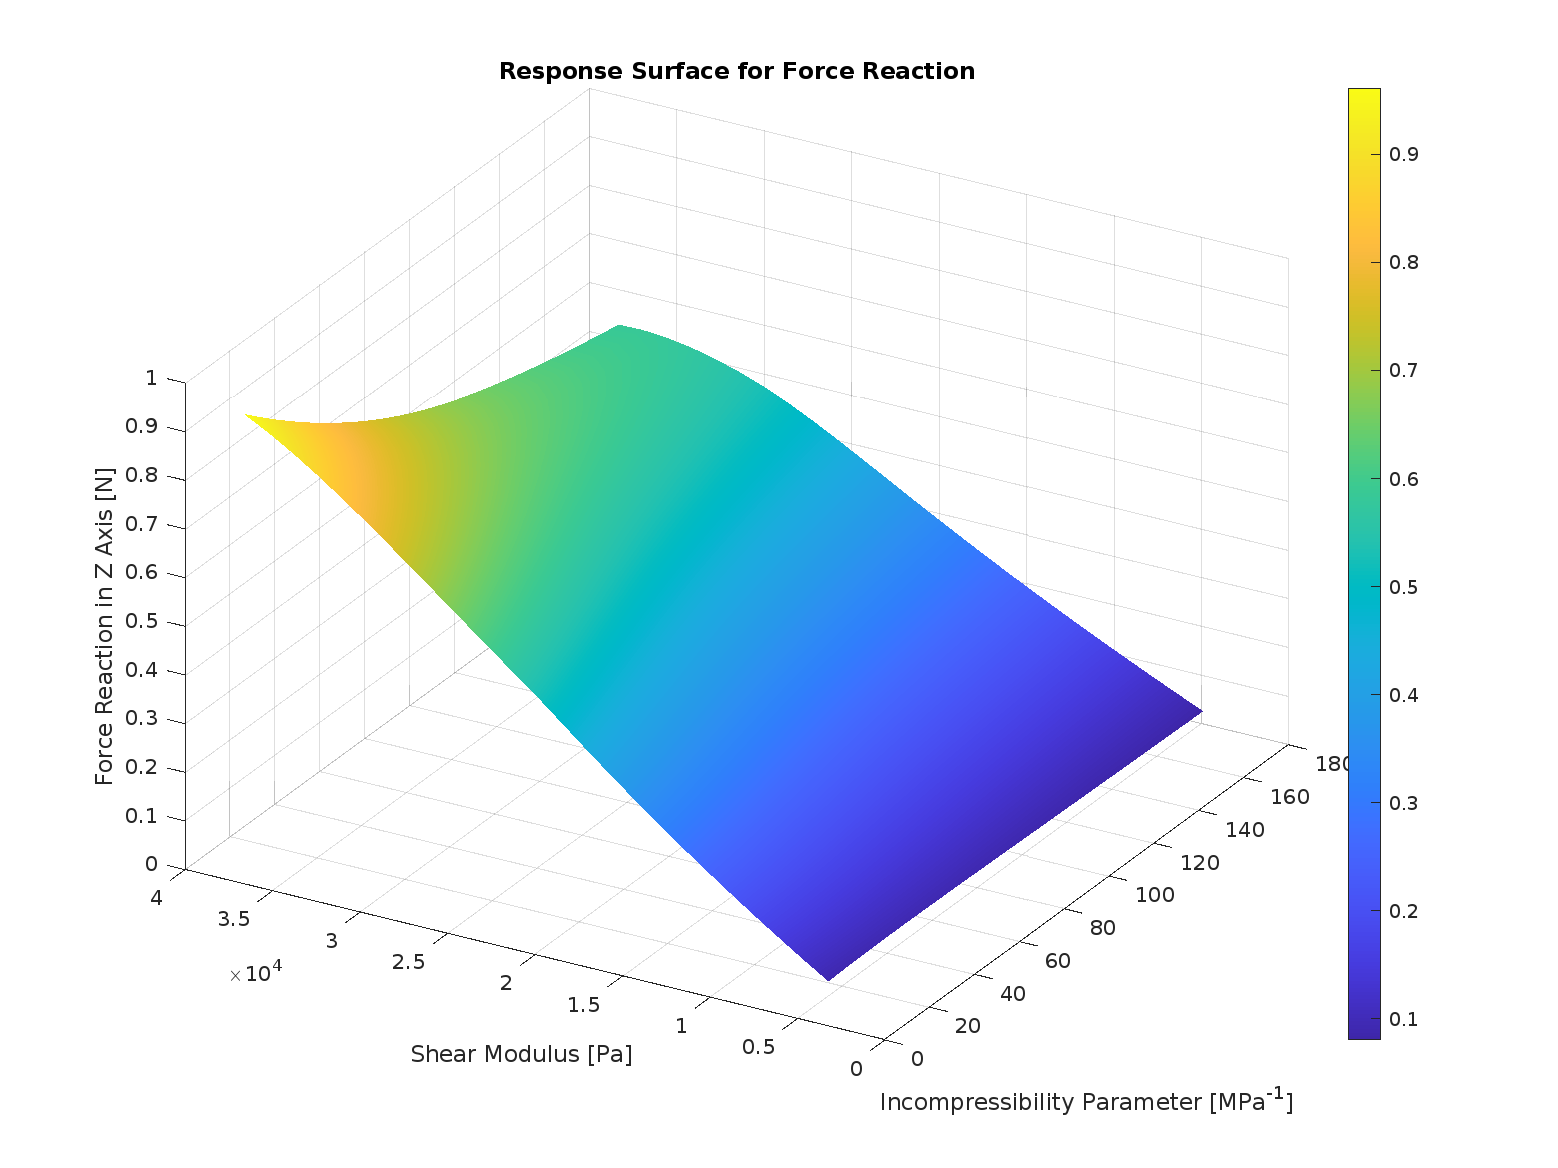
\includegraphics[width=10cm]{Images/ifem/plat NH 4 and 2 fullrange/rsoforce1.png}%
   \caption[Response surface - Force Reaction]{Response Surface for the Neo-Hookean parameters $\mu$ and $D_1$ in relation to the force reaction in the Z-axis.}%
   \label{fig:rsoforce}%
\end{figure}

\subsection*{Initial RSO Results and Evaluation}
The primary performance metric or objective for the RSO was to match the maximum force in the Z-direction, 
observed experimentally at a displacement of $u_z=\SI{4}{\milli\meter}$.
The initial RSO process offered three candidate sets of material parameters, with shear modulus values 
around \SI{0.011}{\mega \pascal} and incompressibility parameter values of \SI{50}{\mega\pascal\tothe{-1}}, 
\SI{112}{\mega\pascal\tothe{-1}}, and \SI{161}{\mega\pascal\tothe{-1}}. Nevertheless, these candidates 
did not match with the experimental maximum force when verified. Moreover, it was observed that ANSYS 
tended to offer only higher values for $D_1$ and ignored the lower half of the range. This led to a decision to 
refine the parameter ranges further.\\

The refined ranges were from \SIrange{7500}{9500}{\pascal} for the shear modulus and 
\SIrange{1}{10}{\mega\pascal\tothe{-1}} for the incompressibility parameter. The new candidates from the RSO had a 
$\mu$ around \SI{0.085}{\mega \pascal} and $D_1$ of \SI{2}{\mega\pascal\tothe{-1}}, 
\SI{5}{\mega\pascal\tothe{-1}}, and \SI{7}{\mega\pascal\tothe{-1}}. 

Furthermore, it was observed that the maximum total deformation of the specimen did not fully reach the  
displacement of \SI{4}{\milli\meter}, therefore a new target was modified and set for a displacement 
of $u_z\approx\SI{3.9}{\milli\meter}$.

\subsection*{Assessment and Process Optimization}
For each simulation curve obtained, the Root Mean Square Error (RMSE) was calculated.
The RMSE is considered a commonly used metric to evaluate the differences between the predicted and 
observed values in the experiments. This function measured the standard deviation of the residuals 
or prediction errors. The RMSE is given by the formula 
\begin{align}
	\text{RMSE} = \sqrt{\frac{1}{n}\sum_{i=1}^{n}(y_i - \hat{y}_i)^2}\, ,
\end{align}
where $y_i$ is the observed or experimental value, $\hat{y}_i$ is the predicted or simulated value, and 
$n$ is the number of data points. However, since the RMSE is scale-dependent, it was normalized by dividing the
RMSE value with the difference of the maximal and minimal value of the observed data
\begin{align}
	\text{NRMSE} = \frac{\text{RMSE}}{y_{max} - y_{min}} \, .
\end{align}

Although the RSO proved to be useful, the obtained candidates were not providing a satisfactory 
match to the entire load-displacement curve when using only a single point as the optimization target.
%buscar un ejemplo con un grafico mostrando dos puntos y un punto
%explicar cambio en sets

\subsection{Minimizing the Objective Function}

In addition to the RSO, a separate optimization was conducted in MATLAB to find the global minimum of the objective function. The objective function was defined as the NRMSE, which quantifies the difference between the simulated and experimental responses.

The MATLAB optimization used the data from the RSO to approximate the objective function as a surface in a three-dimensional space. The x-axis represented the shear modulus, the y-axis represented the incompressibility parameter, and the z-axis represented the NRMSE of each simulation.

The MATLAB optimization then used a mathematical algorithm (such as gradient descent or a genetic algorithm) to search this surface for the set of input parameters that minimized the NRMSE. This set of parameters represented the optimal solution that best matched the experimental data.

This was a bit more detailed explanation of those aspects. Please let me know if you'd like to delve into any other specific areas or if you have further queries.


Additionally, an effort was made to find the global minimum of the objective function (the relationship between the input parameters and the NRMSE) using MATLAB. Using data from approximately 40 simulations, a surface was approximated where the x-axis represented the shear modulus, the y-axis represented the incompressibility parameter, and the z-axis represented the NRMSE of each simulation. The Mean Relative Error (MRE) was also calculated for each simulation, and the same surface approximation method was applied.

\section{Evaluation of the Identified Material Parameters}

The material parameters identified through the RSO and the MATLAB-based optimization were introduced into the computational model for evaluation. The performance of these parameter sets was compared against the experimental data to determine their adequacy.


\section{Comparison between RSO and MATLAB Optimization}

Both RSO and MATLAB-based optimization are valuable tools for parameter estimation and can offer unique advantages in different scenarios. Here, we outline the strengths and weaknesses of each method based on the experiences in this study.

\textbf{Strengths of RSO:}

	1. \textit{User-Friendly Interface:} RSO in ANSYS provides a relatively user-friendly interface that does not require advanced knowledge of programming languages. This can make the process more accessible for users who do not have a background in programming.
	2. \textit{Integrated Design:} Since RSO is an integral part of ANSYS, it works seamlessly with the rest of the software package. This integration can streamline the workflow and reduce the likelihood of errors or inconsistencies.
	3. \textit{Sensitivity Analysis:} RSO includes built-in tools for sensitivity analysis, which can provide valuable insights into the relative importance of each input parameter.

\textbf{Weaknesses of RSO:}

	1. \textit{Limited Flexibility:} RSO may offer less flexibility compared to custom-coded MATLAB optimization routines. For example, it might not be possible to use custom objective functions or optimization algorithms.
	2. \textit{Inability to Handle Complex Objective Functions:} RSO can struggle with objective functions that are highly nonlinear, discontinuous, or have multiple local minima.

\textbf{Strengths of MATLAB Optimization:}

	1. \textit{Highly Customizable:} MATLAB allows for highly customizable optimization routines. You can design your own objective function, constraints, and choose from a variety of optimization algorithms.
	2. \textit{Advanced Analysis Tools:} MATLAB provides advanced tools for data analysis and visualization, which can be useful for interpreting the results of the optimization.

\textbf{Weaknesses of MATLAB Optimization:}

	1. \textit{Requires Programming Knowledge:} Unlike RSO, MATLAB-based optimization requires a good understanding of programming, which can be a barrier for some users.
	2. \textit{Separate Workflow:} Since MATLAB is a separate software, it requires an additional step of exporting and importing data between ANSYS and MATLAB. This can add complexity to the workflow.

In conclusion, the choice between RSO and MATLAB optimization depends on the specific requirements of the study, the complexity of the problem, and the resources and skills available. In this study, both methods were used to leverage their unique advantages and to provide a more comprehensive parameter estimation.



%\section{Material Modeling}
%In an ideal and first scenario, this material can be assumed as linear, isotropic, 
%elastic and nearly imcompressible. For this case, there are two main variables, the Young's
%Modulus \(E\), and the Poisson's ratio $\nu$.
%
%%comentario sobre la influencia del bulk modulus y poissons ratio
%From the parametric analysis, it is possible to see that the bulk 
%modulus of this material does not possess a big impact in the FE 
%simulation results. This conclusion combined with the results 
%from the Poisson ratio in the first material model coincide with the 
%statements from Bergström, where it is no vital to know these parameters 
%to obtain accurate FE computational models, as these have limited
%influence on the mechanical response. \cite{Bergström2015} %pag64Bergströom




%----------------------------------------------------------------------------------
%\subsection{Objective Function Optimzation}

%\subsection{Analysis and Comparison of Each Approach}

%---------------------------------------------------------------------------------
